\chapter{Feature extraction}\label{chap:feature_extraction}
Key primitives in a vision system are low-level filters, such as convolution with Gaussian or edge filters. These filters turn images into maps that indicate the presence of certain frequencies and colors, or help in suppressing unwanted information. A next step before arriving at semantic information such as ``this is a cup'' or ``this is a horse'', is identifying higher-level features that consist of some combination of frequency and color information. 

The goal of this chapter is to introduce a series of standard feature detectors such as the 
\begin{itemize}
\item Hough-transform to detect lines, circles and other shapes,
\item numerical methods such as least-squares, split-and-merge and RANSAC to find high-level features in noisy data,
\item Scale-invariant features.
\end{itemize}

\section{Feature detection as an information-reduction problem}
The information generated by sensors can be quite formidable. For example, a simple webcam generates 640x480 color pixels (red, green and blue) or 921600 Bytes around 30 times per second. A single-ray laser scanner still provides around 600 distance measurements 10 times per second. This is in contrast to the information that a robot actually requires. Consider for example the maze-solving competition ``Ratslife'' (Section \ref{sec:ratslife}) in which the robot's camera can be used to recognize one of 48 different color patterns (Figure \ref{fig:ratslife}) that are distributed in the environment, or the presence or absence of a charger, essentially reducing hundreds of bytes of camera data to around 6 bit ($2^6=64$ different values) content. The goal of most image processing algorithms is therefore to first reduce information content in a meaningful way and then extract relevant information. In chapter \ref{chap:vision}, we have seen convolution-based filters such as blurring, detecting edges, or binary operations such as thresholding. We are now interested in methods to extract higher-level features such as lines and techniques to extract them.

\section{Features}
Lines are particularly useful features for localization and can correspond to walls in laser scans, markers on the floor or corners detected in a camera image. Whereas a Sobel filter (Section \ref{sec:sobel}) can help us to highlight lines and edges in images, additional algorithms are needed to extract structured information such as the orientation and position of a line with respect to the robot.

A desirable property of a feature is that its extraction is repeatable and robust to rotation, scale, and noise in the data. We need feature detectors that can extract the same feature from sensor data, even if the robot has slightly turned or moved farther or closer to the feature. There are many feature detectors available that accomplish this, prominent examples are the Harris corner detector\index{Harris Corner Detector} (essentially detecting points in the image where vertical and horizontal lines cross) and the SIFT feature detector\index{SIFT features}. Feature detection is important far beyond robotics and is for example used in hand-held cameras that can automatically stitch images together. Here, feature detectors will ``fire'' on the same features in two images taken from slightly different perspectives, which allows the camera to calculate the transformation between the two. 

This chapter focuses on two important classes of features: line features and scale-invariant features in images (SIFT). Both features provide tangible example for the least-squares and RANSAC algorithms, which are also introduced in this chapter. Both features are representative for a large class of detectors, and have been chosen for their simplicity, providing a basis for understanding the function of more complex feature detectors. 

\section{Line recognition}
Why are lines a useful feature? As you will see next chapter, the key challenge in estimating a robot's pose is unreliable odometry, in particular when it comes to turning. Here, a simple infrared sensor measuring the distance to a wall can provide the robot with a much better feel for what actually happened. Similarly, if a robot has the ability to track markers in the environment using vision, it gets another estimate on how much it is actually moving. How information from odometry and other sensors can be fused not only to localize the robot, but also to create maps of its environment, will be the focus of the remainder of this book.

A laser scanner or similar device pointed against a wall will return a suite of $N$ points at position $(x_i,y_i)$ in the robot's coordinate system. These points can also be represented in polar coordinates $ (\rho_i,\theta_i)$. We can now imagine a line running through these points that is parametrized with a distance $r$ and an angle $\alpha$. Here, $r$ is the distance of the robot to the wall and $ \alpha$ its angle. As all sensors are noisy, each point will have distance $d_i$ from the ``optimal'' line running through the points. These relationships are illustrated in Figure \ref{fig:linefitting}.
\begin{figure}
	\centering
		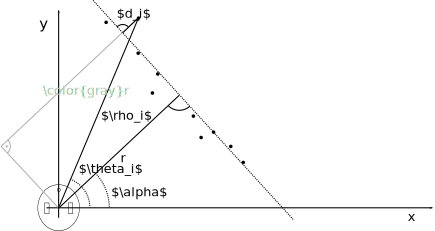
\includegraphics[width=\textwidth]{figs/linefitting.png}
	\caption{A 2D point cloud recorded by a laser-scanner or similar device. A line (dashed) is fitted through the points in a least-square sense.}
	\label{fig:linefitting}
\end{figure}

\subsection{Line fitting using least squares}
Using simple trigonometry we can now write
\begin{equation}
\rho_i \cos(\theta_i-\alpha)-r=d_i.
\end{equation}

Different line candidates --- parametrized by $ r$ and $ \alpha$ --- will have different values for $ d_i$. We can now write an expression for the total error $ S_{r,\alpha}$ as

\begin{equation}
S_{r,\alpha}=\sum_i{d_i^2}=\sum_i(\rho_i \cos(\theta_i-\alpha)-r)^2
\end{equation}

Here, we square each individual error to account for the fact that a negative error, i.e.\ a point left of the line, is as bad as a positive error, i.e.\ a point right of the optimal line. In order to optimize $ S_{r,\alpha}$, we need to take the partial derivatives with respect to $ r$ and $ \alpha$, set them zero, and solve the resulting system of equations for $ r$ and $ \alpha$.

\begin{equation}
\frac{\partial{S}}{\partial{\alpha}}=0 \qquad \frac{\partial{S}}{\partial{r}}=0
\end{equation}

Here, the symbol $ \partial$ indicates that we are taking a partial derivative. Solving for $r$ and $\alpha$ is involved, but possible \cite{siegwart2011introduction}:

\begin{equation}
\alpha=\frac{1}{2}atan2\left(\frac{\sum{\rho_i^2 sin 2\theta_i}-\frac{2}{i}\sum{\sum{\rho_i,\rho_j cos \theta_i sin \theta_j}}}{\sum{\rho_i^2 cos 2 \theta_i - \frac{1}{i}\sum{\sum{\rho_i \rho_j cos(\theta_i+\theta_j)}}}}\right)
\end{equation}

and
\begin{equation}
r=\frac{\sum \rho_i cos (\theta_i-\alpha)}{i}
\end{equation}

We can therefore calculate the distance and orientation of a wall captured by our proximity sensors relative to the robot's positions or the height and orientation of a line in an image based on a collection of points that we believe might belong to a line.

This approach is known as the \emph{least-square method}\index{Least-Square Method (Line fitting)} and can be used to fit data to any parametric model. The general approach is to describe the fit between the data and the model in terms of an error. The best fit will minimize this function, which will therefore have a zero derivative at this point. If the result cannot be obtained analytically as in this example, numerical methods have to be used to find the best fit that minimizes the quadratic error.

\subsection{Split-and-merge algorithm}
A key problem with this approach is that it is often unclear how many lines there are and where a line starts and where it ends. Looking through the camera, for example, we will see vertical lines corresponding to wall corners and horizontal ones that correspond to wall-floor intersections and the horizon; using a distance sensor, the robot might detect a corner. We therefore need an algorithm that can separate point clouds into multiple lines. One possible approach is to find the outlier with the strongest deviation from a fitted line and split the line at this point. This is illustrated in Figure \ref{fig:splitandmerge}. This can be done iteratively until each line has no outliers above a certain threshold. 

\begin{figure}
\includegraphics[width=\textwidth]{figs/splitandmerge}
\caption{Split-and-merge algorithm. Initial least-square fit of a line (left). Splitting the data-set at the point with the highest error (after picking a direction) allows fitting two lines with overall lesser error.\label{fig:splitandmerge}} 
\end{figure}

\subsection{RANSAC: Random Sample and Consensus}
If the number of ``outliers'' are large, a least square fit will generate poor results as it will generate the ``best'' fit that accomodates both ``inliers'' and ``outliers''. Also, split-and-merge algorithms will fail as they are extremely susceptive to noise: depending on the actual parameters every outlier will split a potential line into two. A solution to this problem is to randomly sample possible lines and keep those that satisfy a certain desired quality given by the number of points being somewhat close to the best fit. This is illustrated in Figure \ref{fig:ransac}, with darker lines corresponding to better fits. RANSAC\index{RANSAC}\index{Random Sample and Consensus} usually requires two parameters, namely the number of points required to consider a line to be a valid fit, and the maximum $d_i$ from a line to consider a point an inlier and not an outlier. The algorithm proceeds as follows: select two random points from the set and connect them with a line. Grow this line by $d_i$ in both directions and count the number of inliers. Repeat this until one or more lines that have sufficient number of inliers are found, or a maximum number of iterations are reached.

\begin{figure}
\center
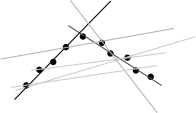
\includegraphics[width=0.6\textwidth]{figs/ransac}
\caption{Random Sample and Consensus (RANSAC). Random lines are evaluated by counting the number of points close by (''inliers''), darker lines are better fits.\label{fig:ransac}} 
\end{figure}

The RANSAC algorithm is fairly easy to understand in the line fitting application, but can be used to fit arbitrary parametric models to any-dimensional data. Here, its main strength is to cope with noisy data.

Given that RANSAC is random, finding a really good fit will take quite some time. Therefore, RANSAC is usually used only as a first step to get an initial estimate, which can then be improved by some kind of local optimization, such as least-squares, e.g.

\subsection{The Hough Transform}
The Hough transform \index{Hough transform} can best be understood as a voting scheme to guess the parametrization of a feature such as a line, circle or other curve \cite{duda1972use}. For example, a line might be represented by $y=mx+c$, where $m$ and $c$ are the gradient and offset. A point in this parameter space (or ``Hough-space'') then corresponds to a specific line in $x-y$-space (or ``image-space''). The Hough-transform now proceeds as follows: for every pixel in the image that could be part of a line, e.g., white pixels in a thresholded image after Sobel filtering, construct all possible lines that intersect this point. (Drawing an image of this would look like a star). Each of these lines has a specifc $m$ and $c$ associated with it, for which we can add a white dot in Hough-space. Continuing to do this for every pixel of a line in an image will yield many $m-c$ pair, but only one that is common among all those pixels of the line in the image: the actual $m-c$ parameters of this line. Thinking about the number of times a point was highlighted in Hough-space as brightness, will turn a line in image space into a bright spot in Hough-space (and the other way round). In practice, a polar representation is chosen for lines. This is shown in Figure \ref{fig:hough}. The Hough transform also generalizes to other parametrization such as circles.  

\begin{figure}
\center
\includegraphics[width=\textwidth]{figs/houghtransform}
\caption{Lines in an image (left) transposed into Hough-space $\rho$ (distance from origin) and $\theta$ (angle of normal with respect to origin). Bright spots in the Hough image (right) correspond to parameters that have received the most ``votes'' and clearly show the two lines at around 90$^o$ and 180$^o$.\label{fig:hough}} 
\end{figure}


\section{Scale-Invariant Feature Transforms}
Scale-invariant feature transforms are a class of algorithms/signal-processing techniques that allow to extract features that are easily detectable across different scales (or distances to an object), independent of their rotation, and to some extent robust to affine transformations, i.e., views of the same object from different perspectives, and illumination changes. The most prominent in this class is the SIFT algorithm \cite{lowe1999object},\index{SIFT} which however has lost popularity due to closed-source and licensing cost, and has been replaced in the past with SURF (Speed-Up Robust Feature)\index{SURF} and many others,  which are freely available and have slightly different performance and varying use cases. As the math behind SURF is more involved, we focus on the intuition behind SIFT and encourage the reader to download and play with the various open-source implementations of other feature detectors that are available open source.

\subsection{Overview}
SIFT proceeds in multiple steps. Descriptions of the algorithm often include its application to object recognition, but these algorithms are independent of feature generation (see below).

\begin{enumerate}
\item Differences of Gaussians (DoG) at different scales:
\begin{itemize}
\item Generate multiple scaled versions of the same image by re-sampling every 2nd, 4th and so on pixel.
\item Filtering each scaled picture with various Gaussian filters of different variance.
\item Calculating the difference between pairs of filtered images. This is equivalent to a DoG filter.
\end{itemize}

\item Detecting local minima and maxima in the DoG images across different scales (Figure \ref{fig:siftrejection}, left) and reject those with low contrast (Figure \ref{fig:siftrejection}, right). 

\begin{figure}
	\centering
		\includegraphics[width=\textwidth]{figs/siftrejection.png}
	\caption{After scale space extrema are detected (left), the SIFT algorithm discards low contrast keypoints (center) and then filters out those located on edges (right). \copyright Lukas Mach CC-BY 3.0}
	\label{fig:siftrejection}
\end{figure}

\item Reject extrema that are along edges by looking at the second derivative around each extrema (Figure \ref{fig:siftrejection}, right). Edges have a much larger principal curvature across them than along them.
\item Assign a ``magnitude'' and ``orientation'' to each remaining extrema (keypoint). The magnitude is the squared difference between neighboring pixels and the orientation is the angle between magnitude along the y-axis vs. magnitude along the x-axis. These calculations are made for all pixels in a fixed neighborhood around the initial keypoint, e.g., in a 16x16 pixel neighborhood.
\item Collect orientations of neighboring pixels in a histogram, e.g., 36 bins each covering 10 degrees. Maintain the orientation corresponding to the strongest peak and associate it with the keypoint.
\item Repeat step 4, but for four 4x4 pixel areas around the keypoint in the image scale that has the most extreme minima/maxima. Here, only 8 bins are used for the orientation histogram. As there are 16 histograms in a 16x16 pixel area, the feature descriptor has 128 dimensions.
\item The feature descriptor vector is normalized, tresholded, and again normalized to make it more robust against illumination changes.
\item Local gradient magnitude and orientation are grouped into bins and create a 128-dimensional feature descriptor.
\end{enumerate}

The resulting 128 dimensional feature vectors are now scale-invariant (due to step 2), rotation-invariant (due to step 5), and robust to illumination changes (due to step 7).

\subsection{Object Recognition using scale-invariant features}
Scale-invariant features of training images can be stored in a database and can be used to identify these objects in the future. This is done by finding all features in an image and comparing them with those in the database. This comparison is done by using the Euclidian distance as metric and searching a k-d tree (with d=128). In order to make this approach robust, each object needs to be identified by at least 3 independent features. For this, each descriptor stores the location, scale and orientation of it relative to some common point on the object. This allows each detected feature to ``vote'' for the position of the object that it is most closely associated with in the database.  This is done using a Hough-transform. For example, position (2 dimensions) and orientation (1 dimension) can be discretized into bins (30 degree width for orientation); bright spots in Hough-space then correspond to an object pose that has been identified by multiple features.

\section*{Take-home lessons}
\begin{enumerate}
\item Features are ``interesting'' information in sensor data that are robust to variations in rotation and scale as well as noise
\item Which features are most useful depends on the characteristics of the sensor generating the data, the structure of the environment, and the actual application.
\item There are many feature detectors available some of which operating as simple filters, others relying on machine learning techniques.
\item Lines are among the most important features in mobile robotics as they are easy to extract from many different sensors and provide strong clues for localization.
\end{enumerate}

\section*{Exercises}\small
\begin{enumerate}
\item Think about what information would make good features in different operating scenarios: a supermarket, a warehouse, a cave. 
\item What other features could you detect using a Hough transform? Can you find parameterizations for a circle, a square or a triangle?
\item Do an online search for SIFT. What other similar feature detectors can you find? Which provide source code that you can use online?
\item A line can be represented by the function $y=mx+c$. Then, the Hough-space is given by a 2D coordinate system spanned by $m$ and $c$.\begin{enumerate}
\item Think about a line representation in polar coordinates. What components has the Hough-space in this case?
\item Derive a parameterization for a circle and describe the resulting Hough space.
\end{enumerate}
\end{enumerate}
\normalsize